\documentclass[10pt]{SPIIRAS_Proceedings}

\graphicspath{{media/}}

\usepackage{subfig}
\usepackage{tikz}
\usetikzlibrary{patterns,intersections}

\usepackage{enumitem}

\usepackage[%
  parentracker=true,
  style=gost-numeric,
  defernumbers=true,
  sorting=none,
]{biblatex}

% \toggletrue{bbx:gostbibliography}

\addbibresource{ccp.bib}

\udk{519.8.А}

\titleRus{
  Новый алгоритм построения кратчайшего пути обхода
  конечного множества непересекающихся контуров на плоскости
}

\authorsRus{
  А.А. Петунин,
  Е.Г. Полищук,
  С.С. Уколов.
}

\authorsTitleRus{
  А.А. П\smallcapsfake{етунин},
  Е.Г. П\smallcapsfake{олищук},
  С.С. У\smallcapsfake{колов}
} % \smallcapfake необходим для имитации малых прописных букв ввиду отсутствия поддержки в используемом шрифте

\abstractRus{
  Рассматривается проблема маршрутизации режущего
  инструмента машин термической резки с ЧПУ
  когда точки врезки расположены
  на границах деталей,
  ограниченных отрезками прямых и дугами окружностей
  с использованием техники непрерывной резки
  (CCP),
  то есть каждый контур вырезается целиком.
  Общая задача минимизации длины маршрута
  в этом случае сводится к минимизации длины холостого хода.
  Показано, что она эквивалентна поиску
  кратчайшей ломаной с вершинами,
  расположенными на контурах.
  Представлен алгоритм построения
  такой ломаной для заданного порядка
  обхода контуров,
  доставляющий локальный минимум
  а также предложены достаточные условия
  глобального минимума.
  Предложен эвристический алгоритм
  маршрутизации на основе
  метода переменных окрестностей
  (VNS).
  Рассмотрены результаты численных экспериментов
  в сравнении с точным решением задачи GTSP.
}

\keywordsRus{
  задача резки,
  непрерывная резка,
  оптимизация,
  достаточные условия,
  эвристика,
  GTSP,
  метод переменных окрестностей
}

\begin{document}

\maketitle

\normalsize

\section*{Введение}
\label{sec:intro}

В процессе разработки управляющих программ
для машин термической резки листового материала с ЧПУ
возникает несколько оптимизационных задач.
Одна из них -- минимизация
длины холостого хода инструмента.
Она в некоторых случаях может быть сведена
к задаче поиска кратчайшей ломаной,
вершины которой расположены на заданных
плоских контурах,
являющихся границами деталей.
Расположение этих контуров на плоскости
в свою очередь получено решением другой
оптимизационной задачи -- <<раскроя>>.
Обе упомянутые задачи являются NP-полными.

Задача минимизации длины холостого хода инструмента
сама по себе является частным случаем
общей оптимизационной проблемы
маршрутизации инструмента.
Её полное решение в общем случае
не может быть получено
в разумное время
для задач типичных для современного
промышленного производства
(сотни / тысячи контуров),
поэтому на практике применяются разнообразные эвристики,
дающие решения приемлемого качества.

Для полного решения задачи маршрутизации
режущего инструмента для машин листовой резки
с ЧПУ
для минимизации времени или стоимости резки
требуется решить целый ряд задач.
Их описание и классификация приведены подробно в
\cite{bi01,bi02,bi03},
и схематически изображены на рис.~\ref{CP-classes}.

\begin{itemize}
  \item
  \textbf{Задача непрерывной резки}
  (Continuous Cutting Problem, CCP):
  каждый контур
  (ограничивающий одну из деталей)
  вырезается за один раз,
  одним движением инструмента,
  но резка может начаться в любой точке контура
  (и заканчивается в ней же)

  \item
  \textbf{Обобщённая задача коммивояжера}
  (Generalized Traveling Salesman Problem, GTSP):
  резка может начаться в одной из заранее
  заданных точек на контуре
  (количество таких точек конечно),
  после этого контур вырезается целиком

  \item
  \textbf{Задача резки с остановками}
  (Endpoint Cutting Problem, ECP):
  резка контура может начинаться только в
  заранее заданных точках на нём,
  но контур может вырезаться за несколько раз,
  частями

  \item
  \textbf{Сегментная задача непрерывной резки}
  (Segment Continuous Cutting Problem, SCCP):
  вводится понятие сегмента
  как обобщение понятия контура;
  сегмент может быть частью контура
  или объединением нескольких контуров
  и / или их частей.
  Каждый сегмент вырезается целиком,
  от начала до конца,
  таким образом
  $ CCP \subset SCCP$.

  \item
  \textbf{Обобщённая сегментная задача непрерывной резки}
  (Generalized Segment Continuous Cutting Problem, GSCCP):
  подобна сегментной задаче непрерывной резки
  (SCCP),
  но разбивка на сегменты не задана заранее
  и сама подлежит оптимизации

  \item
  \textbf{Задача прерывистой резки}
  (Intermittent Cutting Problem, ICP):
  наиболее общая формулировка задачи резки,
  встречающаяся в научной литературе,
  контуры могут вырезаться частями,
  в несколько подходов,
  начиная с произвольной точки.
\end{itemize}

\begin{figure}
  \centering
  \def\svgwidth{\columnwidth}
  \input{media/classes.pdf_tex}
  \caption{Классификация задач резки}
  \label{CP-classes}
\end{figure}

На практике задача оптимизации маршрута режущего инструмента
зачастую сводится к дискретной оптимизации
за счёт выбора конечного множества возможных точек врезки
на контурах деталей с некоторым заранее заданным шагом
$\varepsilon$,
то есть сводится к задаче ECP
\cite{bi04,bi05,bi06}
и её частному случаю ---
GTSP
\cite{bi07,bi08,bi09,bi10}.
Задача непрерывной резки CCP
тоже может сводиться к GTSP,
в этом случае суммарная ошибка длины
холостого хода оценивается как
$N \cdot \varepsilon$,
где $N$ -- количество контуров.
Для достижения точности результата
$\delta$,
таким образом необходимо выбирать малое
$\varepsilon \approx \delta / N$,
так что полное количество допустимых точек врезки растёт
(как $O (N)$)
и полный перебор требует экспоненциального времени.
Тем не менее, этот класс задач может успешно решаться,
например,
средствами динамического программирования
(DP)
а для небольших
$N \approx 30$ -- даже точно
(см. в частности \cite{bi15}).

В данной работе рассматриваются вопросы
поиска оптимального маршрута без
применения дискретизации
(то есть задача CCP),
которые слабо освещены в
открытых источниках,
см. например
\cite{bi11,bi12},
где описаны некоторые эвристики.

\subsection*{Технологические ограничения}

Тот факт, что полученный маршрут
должен быть физически выполнен
на конкретной машине термической резки с ЧПУ,
накладывает на последний определённые
технологические ограничения.

Так называемое <<ограничение предшествования>>
(наиболее подробно описанное в литературе),
вызвано тем,
что после вырезания замкнутого контура,
его содержимое более ничем не удерживается
и может свободно вращаться, сдвигаться и даже падать.
Поэтому внутренние контура деталей должны вырезаться до того,
как будет завершена резка содержащих их внешних контуров.
Аналогично и детали, размещённые в отверстиях
других деталей,
также должны вырезаться до завершения резки
содержащих их контуров.

Наконец, технология резки в большинстве случаев
диктует, что резак не может двигаться прямо по контуру детали,
но с некоторым сдвигом
(несколько миллиметров).
Этот сдвиг может вычисляться как в ходе
решения задачи маршрутизации,
так и после -- при генерации управляющей программы
на основе полученного маршрута или даже
непосредственно на станке в процессе резки.
Более того,
точки врезки
(в которых начинается резка)
как правило должны находиться
на ещё большем расстоянии от контуров деталей
во избежание повреждения последних.
В данной работе эти вопросы,
тем не менее,
не рассматриваются,
то есть строится маршрут,
проходящий в точности по контурам деталей,
и точки врезки
(а равно и точки окончания резки и выключения инструмента)
также ищутся прямо на контурах деталей.

\section{Задача непрерывной резки}

Рассмотрим Эвклидову плоскость
$\mathbb R ^ 2$
и на ней фигуру
$B$
(в большинстве практических случаев -- прямоугольник),
ограниченную замкнутым контуром.
Это -- модель листового материала,
подлежащего резке.
Пусть
$N$
попарно непересекающихся плоских контуров
$\{C_1, C_2, ... C_N\}$
расположены внутри
$B$,
ограничивая
$n$
деталей
$\{A_1, A_2 ... A_n\}$.
Деталь может быть ограничена
одним или несколькими контурами
(одним внешним и несколькими отверстиями),
так что в общем случае
$n \leqslant N$.

Контуры
$C_i$
могут быть произвольной формы,
но мы будем рассматривать только
состоящие из
(конечного числа)
отрезков прямых линий и дуг окружностей,
так как именно такие геометрические примитивы
поддерживаются программным обеспечением
современных машин термической резки с ЧПУ.
Частный случай,
когда контура состоят только
из отрезков прямых,
сводится к одному из вариантов
задачи обхода прямоугольников
(Touring Polygon Problem, TPP),
см.
\cite{bi13}.

Далее,
внутри
$B$
(как правило, на границе)
выберем две точки и обозначим их
$M_0$, $M_{N + 1}$
(почти всегда $M_0 = M_{N + 1}$),
которые будут использоваться
как начало и конец
маршрута резки.

Задача непрерывной резки
(Continuous Cutting Problem, CCP)
состоит в поиске:
\begin{enumerate}
\item
$N$ штук точек врезки $M_i \in C_i, i \in \overline{1, N}$
\item
Последовательности обхода контуров
$C_i$,
то есть перестановки
$N$
элементов
$I = (i_1, i_2, ... i_N)$
\end{enumerate}

Результатом решения задачи будет являться маршрут
\begin{equation}
  \{M_0, M_{i_1}, M_{i_2}, \dots M_{i_N}, M_{N + 1}\}
\end{equation}

Целевая функция в данном случае сильно упрощается
по сравнению с общей задачей маршрутизации резки
и сводится фактически к минимизации длины холостого хода:

\begin{equation}
  \mathcal{L} = \sum_{j=0}^N|M_{i_j}M_{i_{j+1}}|
  \label{air-move-length}
\end{equation}
$$
\mathcal{L} \to \min
$$
где, для простоты записи мы полагаем
$M_{i_0} = M_0$,
$M_{i_{N + 1}} = M_{N + 1}$.

Кроме того,
мы потребуем,
чтобы искомое решение задачи
удовлетворяло
описанному выше
ограничению предшествования.

Хотя контуры
$C_i$
по условию не пересекаются,
они могут быть вложены друг в друга:
\( \tilde C_a \subset \tilde C_b \),
где
$\tilde C_a$
обозначает 2-мерную фигуру,
ограниченную контуром
$C_a$
(в более традиционных обозначениях
$C_a = \partial \tilde C_a$).
В общей задаче маршрутизации
режущего инструмента это
соответствует двум разным случаям
(наличие отверстий в деталях с одной стороны
и размещение меньших деталей в отверстиях больших),
но в нашем случае оба этих
варианта обрабатываются одинаково.

Если один контур расположен внутри другого,
то внутренний должен быть вырезан
(посещён)
ранее, чем внешний:
\( \tilde C_a \subset \tilde C_b \Rightarrow i_a < i_b \),
в перестановке
$I = (i_1, i_2, ... i_N)$.
Таким образом,
множество допустимых перестановок ограничено.

\section{Алгоритм CCP-Relax решения задачи непрерывной резки}
\label{sec:ccp-relax}

Предлагаемый алгоритм решения задачи непрерывной резки
(см. \cite{berlin2019})
состоит из нескольких шагов,
что хорошо соответствует самой природе
решаемой задачи.

\subsection{Удаление <<внешних>> контуров}

Для автоматического соблюдения
ограничения предшествования,
мы начинаем с удаления всех контуров,
внутри которых есть вложенные контура,
так, чтобы остались только:
$$
\{C_i | \forall j \ne i: C_j \cap \tilde C_i = \varnothing \}
$$

В общем случае это приводит к уменьшению
(в некоторых случаях -- существенному)
сложности задачи
(с $N$ до некоторого $N'$),
что в свою очередь
сокращает время счёта
на втором и в особенности третьем
шагах алгоритма.

\subsection{Непрерывная оптимизация}

На этом этапе мы полагаем,
что последовательность обхода контуров
$I = (i_1, i_2, ... i_N)$
задана (фиксирована)
и ищем координаты точек врезки
$M_i \in C_i$
во все контура,
минимизируя полную длину холостого хода
(\ref{air-move-length}).
Для этого,
начальные позиции точек врезки выбираются
произвольным образом
(например, случайно)
и затем положение одной (каждой) из точек
$M_i$
изменяется, а все остальные остаются неподвижны:
$\mathcal{L}(M_i) \to \min$.
Большинство слагаемых в целевой функции
(\ref{air-move-length})
при этом постоянны,
так что сама функция упрощается до
$$
|M_{i-1}M_i|+|M_iM_{i+1}| \to \min_{M_i \in C_i}
$$

Несложный геометрический анализ показывает,
что если точки
$M_{i-1}$
и
$M_{i + 1}$
расположены по разные стороны сегмента контура
$C_i$,
то оптимальное положение точки врезки
$M_i$
оказывается на пересечении с этим сегментом:
$M_i = M_{i-1} M_{i + 1} \cap C_i$
(если, конечно,
такое пересечение существует;
в противном случае
решением будет один из концов сегмента),
см. рис. \ref{pierce-thru}.

Если же точки располагаются
с одной стороны сегмента,
решение легко находится при помощи
{\it принципа Ферма},
или другими словами правила
<<угол падения равен углу отражения>>
(или опять на одном из концов сегмента),
см. рис. \ref{pierce-fermat}.

\begin{figure}
  \centering
  \subfloat[На пересечении звена ломаной]{
    \label{pierce-thru}
    \tikz[rotate=-12,scale=0.68]{
        \draw[thick,name path=C1]
            (0,5) node[above] {$C_{i-1}$}
            to[bend right] (1,0);
        \draw[thick,name path=C2]
            (3,0) node[below] {$C_i$}
            to[bend right] (3,2);
        \draw[thick,name path=C3]
            (4,3) node[above] {$C_{i+1}$}
            to[bend right] (5,0);
        \path[name path=L0]
            (0,1.5) -- (6,2);
        \path[name path=Lx]
            (0,1) -- (6,1);
        \fill[name intersections={of=C1 and Lx, name=X}]
            (X-1) coordinate(M1) circle(3pt) node[below] {$M_{i-1}$};
        \fill[name intersections={of=C2 and L0, name=X}]
            (X-1) coordinate(M2) circle(3pt) node[below left]{$M_i$};
        \draw[name intersections={of=C2 and Lx, name=X}]
            (X-1) coordinate(M2x) node[below right]{$M'_i$};
        \fill[name intersections={of=C3 and Lx, name=X}]
            (X-1) coordinate(M3) circle(3pt) node[right] {$M_{i+1}$};
        \draw[dashed]
            (M1) -- (M3);
        \draw[thin,-latex]
            (M2)
            to[bend right] (M2x);
    }
  }
  \subfloat[С использованием \textit{принципа Ферма}]{
    \label{pierce-fermat}
    \tikz[rotate=-12,scale=0.68]{
      \draw[thick]
          (0, 0) coordinate(zero) -- (5, 0) coordinate(future) node[right] {$C_i$};
      \fill[black]
          (1.5, 0) circle(3pt) coordinate(middle) node[below left]  {$M_i$}
          (1, 1) circle(3pt) coordinate(from) node[above right] {$M_{i-1}$} ++(-1.5,0) node[above] {$C_{i-1}$}
          (4.5, 2) circle(3pt) coordinate(to) node[above right] {$M_{i+1}$} ++(1.5,0) node[below] {$C_{i+1}$};
      \begin{scope}
          \clip (from) circle(1);
          \draw[thick] (from) ++(0, 3) circle(3);
      \end{scope};
      \begin{scope}
          \clip (to) circle(1.5);
          \draw[thick] (to) ++(3, 4) circle(5);
      \end{scope};
      % \draw[dashed] (from) -- (middle) -- (to);
      \draw[thin] (4.5, -2) circle(0.062) coordinate(mirror) node[right] {$\hat M_{i+1}$};
      \coordinate (opt) at (intersection of zero--future and mirror--from);
      % \draw[thin] (opt) circle(3pt);
      \draw[dotted]
          (mirror) -- (opt)
          (mirror) -- (to);
      \draw[dashed] (from) -- (opt) -- (to);

      \draw[thin,-latex] (middle) to[bend right] (opt) node[below] {$M'_i$};
    }
  }
  \caption{Оптимальное положение точки врезки}
  \label{shift-pierce-point}
\end{figure}

Общая схема этого шага оптимизации может быть записана таким образом:
\begin{enumerate}
  \item
  Выбираем произвольные начальные позиции точек врезки
  $M_i \in C_i, \forall i$.
  \item
  $\forall i \in \overline{1,N}$
  находим оптимальное положение
  $M_i$
  как описано выше за константное время
  \item
  Повторяем предыдущий шаг,
  до тех пор,
  пока длина холостого пути
  (\ref{air-move-length})
  не сойдётся
  (с некоторой наперёд заданной точностью $\delta$)
\end{enumerate}

На практике весь процесс хорошо сходится
за время
$O(N)$
и поэтому многократно применяется
в качестве подпрограммы на следующем шаге.

\subsection{Дискретная оптимизация}

Наиболее вычислительно сложная задача
заключается в поиске перестановки
$I = (i_1, i_2, ... i_N)$,
минимизирующей полную длину холостого хода
$\mathcal{L} \to \min$.
Фактически,
это решение
Задачи коммивояжёра
(Traveling Salesman Problem, TSP),
только длина пути вычисляется
не аддитивно,
а при помощи процесса
непрерывной оптимизации,
описанного на предыдущем шаге.

В данной работе для поиска
такой перестановки применяется
метод переменных окрестностей
(Variable Neighborhood Search,
VNS, см. \cite{bi14})
по такой схеме:

\begin{enumerate}[label*=\arabic*.]
  \item Начальная перестановка
  $I = (i_1, i_2, ... i_N)$
  выбирается произвольным образом
  (например, случайно)
  \item $k=1$
  \item while $k < k_{max}$:
  \begin{enumerate}
    [label*=\arabic*.]
    \item Выбираем перестановку $I' \in \mathcal N^k(I)$
    из окрестности
    $\mathcal N^k(I)$,
    доставляющую минимум
    $\mathcal L(I')$
    \item if $\mathcal L(I')< \mathcal L(I)$:
    \begin{enumerate}[label*=\arabic*.]
      \item $I \gets I'$
      \item $k \gets 1$
    \end{enumerate}
    \item else
    \begin{enumerate}[label*=\arabic*.]
      \item $k \gets k+1$
    \end{enumerate}
  \end{enumerate}
  \item Завершение работы.
\end{enumerate}

На шаге 3.1
многократно применяется
непрерывная оптимизация из предыдущего этапа:
$$
\mathcal L (I') = \min_{M_1, M_2 \dots M_N}
  \mathcal L (M_1, M_2 \dots M_N | I')
$$

Окрестности
$\mathcal N^k(I)$
различного размера
конструируются разнообразными способами,
например:

\begin{itemize}
  \item
  Все возможные парные перестановки
  (то есть, окрестности размера 1 в смысле транспозиционной метрики)
  \item
  Циклические перестановки 3 контуров.
  Поскольку всего таких перестановок получается
  $O (N ^ 3)$,
  выбираются только те из них,
  в которых задействованные контуры расположены
  в исходной перестановке
  $I = (i_1, i_2, ... i_N)$
  не далее, чем на предопределённом расстоянии
  друг от друга;
  это предопределённое расстояние является
  параметром алгоритма
  \item
  Подобным же образом,
  выбираются циклические перестановки 4 контуров,
  лежащих не далее заданного расстояния
  друг от друга в исходной перестановке
  $I = (i_1, i_2, ... i_N)$
  \item
  Выбирается последовательный блок контуров
  произвольной длины и к нему применяется
  циклический сдвиг
  \item
  Все контуры в последовательном блоке
  контуров
  (произвольной длины)
  переставляются в обратном порядке
  \item
  Перестановка двух последовательных
  (но не смежных) блоков контуров
  \item
  Циклическая перестановка нескольких
  последовательно расположенных
  последовательных блоков контуров
  (произвольной но одинаковой длины)
  \item
  И ещё порядка десяти других способов генерации
  <<близких>> к исходной перестановок
\end{itemize}

Если размер некоторой окрестности
$\mathcal N^k(I)$,
получаемой одним из способов,
оказывается слишком большим
(что приводит к увеличению времени счёта),
он легко может быть ограничен
при помощи введения дополнительного параметра
алгоритма,
подобно тому,
как это сделано для тройных
и четверных циклических перестановок.

Кроме того,
сам метод переменных окрестностей
допускает несколько вариантов применения,
например замена полного перебора
(на шаге 3.1)
на <<первый подходящий>>
или метод Монте-Карло,
но их влияние на скорость
и качество получаемого решения
задачи непрерывной резки
требует дальнейшего исследования.

\subsection{Восстановление удалённых контуров}

\begin{figure}
  \centering
  \tikz[scale=0.68]{
    \path
        (-2,0.5) coordinate(M1)
        (-1,1) coordinate(M2)
        (8,2) coordinate (M4)
        (10,4) coordinate (M5);
    ;
    \filldraw[thick,pattern=crosshatch]
        (M2) -- ++(80:1.2) -- ++(170:1.2) -- ++(260:1.2) -- cycle
        (M4) -- ++(260:1.6) -- ++(20:1.6) -- cycle;
    ;
    \filldraw[thick,rounded corners,pattern=crosshatch,even odd rule,name path=Ai]
        (0,0) rectangle (7,4)
        (6,3) rectangle (6.8,3.8)
        (6,1) rectangle (6.8,0.2)
        (2,2) circle(1.6)
    ;
    \path[name path=Lx]
        (M2) -- (M4);
    \path[name intersections={of=Ai and Lx, name=Mi}]
        (Mi-3) coordinate (M3)
        (Mi-2) coordinate (M3_5)
    ;
    \fill
        \foreach \i in {1,...,5} {
            (M\i) circle (2pt)
        }
    ;
    \draw [ultra thick]
        (M3_5) circle(3pt) node[above right] {$M_+$}
    ;
    \draw[thin,-latex]
        (M1) node[below] {$M_1$} --
        (M2) node[below] {$M_2$} --
        (M3) node[above right] {$M_3$} --
        (M4) node[right] {$M_4$} --
        (M5) node[left] {$M_5$}
    ;
  }
  \caption{Добавление точек врезки во <<внешние>> контура $M_+$}
  \label{extra-pierce-point}
\end{figure}

На предыдущем шаге мы получили
последовательность обхода контуров
и точки врезки для каждого из них,
но только для тех,
которые не содержат других контуров внутри себя.
Теперь необходимо дополнить эту последовательность
оставшимися контурами
(удалёнными на первом шаге)
и точками врезки для них,
причём таким образом,
чтобы ограничение предшествования
оказалось соблюдённым.

Заметим, что маршрут,
полученный к этому моменту
\begin{equation}
Route = \{ M_0, M_1, M_2, \dots M_{N'}, M_{N'+1}\}
\label{route0}
\end{equation}
обязательно пересекает все исходные контуры
$C_i$,
потому что для контуров,
сохранённых на первом шаге,
он их явно посещает
по построению шагов 2 и 3,
а для остальных контуров --
ввиду того, что
каждый из них включает в себя
один из посещённых контуров,
а начальная и конечная точка
$M_0$
и
$M_{N + 1}$
всегда выбираются снаружи всех контуров
$C_i$.

Таким образом,
для каждого
<<внешнего>> контура
$C_i$,
который пока не включён в маршрут резки,
мы находим все точки пересечения
с полученным маршрутом
(\ref{route0}),
и если таких точек несколько
(что как правило и бывает),
выбираем из них самую последнюю,
то есть посещаемую маршрутом позже всех
других,
см. рис. \ref{extra-pierce-point}.
Сам контур
$C_i$
вставляется в перестановку
в месте,
соотвествующем выбранной точке врезки.

После добавления таким образом всех
<<внешних>> контуров
и соответствующих им точек врезки,
мы получаем уже полный маршрут,
который посещает все исходные контуры,
причём внутренние контуры посещаются
строго раньше содержащих их внешних.
Полная длина маршрута
при этой операции,
очевидно,
не меняется.

Легко понять,
что получаемый таким образом полный маршрут
является оптимальным решением исходной задачи
непрерывной резки.
Действительно,
если бы существовал более короткий маршрут,
посещающий все контура,
из него можно было бы просто удалить
точки врезки,
лежашие на
<<внешних>> контурах,
получив тем самым маршрут,
обходящий <<внутренние>> контура
и имеющий ту же,
то есть меньшую длину.
Таким образом, существует лучшее
решение для задачи обхода
части контуров без учёта
ограничений предшествования,
но это по предположению невозможно.

Таким образом,
мы строго выполняем
ограничение предшествования,
тратя на это линейное время
$O(N)$.

На этом выполнение
предложенного эвристического алгоритма
решения задачи непрерывной резки
завершается.

\section{Условия оптимальности решения непрерывной задачи}


С практической точки зрения,
вышеописанный алгоритм оказывается
вполне работоспособным
и даёт хорошие результаты,
как в смысле времени работы,
так и качества получаемых решений.
Однако,
это чисто эмпирический результат,
так что было бы интересно получить
теоретические оценки качества работы
данного алгоритма.

Наиболее важным и одновременно
наиболее сложным является,
конечно, третий этап --
дискретная оптимизация
(фактически решение задачи коммивояжёра),
как с теоретической,
так и с практической точки зрения.
В данной же работе исследуется
второй шаг алгоритма --
непрерывная оптимизация.
Оказывается возможным сформулировать
некоторые утверждения относительно
получаемых в её ходе решений.

% \begin{remark}
  На рис. \ref{counter-example}
  показан пример маршрута резки,
  который не являясь кратчайшим,
  тем не менее неё
  может быть приведён к таковому
  никакими индивидуальными сдвигами
  точек врезки.
  Таким образом, возникает вопрос,
  при каких условиях предлагаемый алгоритм
  гарантирует получение действительно
  оптимального маршрута,
  то есть другими словами,
  глобального минимума оптимизационной задачи.
% \end{remark}

\begin{figure}
  \centering
  \begin{tikzpicture}[scale=2.5]
    \draw
      (1,-0.2) node(M3){} circle(0.027) node[below] {$M_3$}
      (-1,-0.2) node(M0){} circle(0.027) node[below] {$M_0$};

    \draw [thick,pattern=crosshatch]
      (-1.3, 0) arc(270:90:0.5) node[midway,right]{$C_1$} -- (-1.0, 1.0) node(M1x){} -- (-1.0, 1.1) -- (-1.3, 1.1) arc(90:270:0.6) node(M1){} -- cycle
      (1.3, 0) arc(-90:+90:0.5) node[midway,left]{$C_2$} -- (1.0, 1.0) node(M2x){} -- (1.0, 1.1) -- (1.3, 1.1) arc(+90:-90:0.6) node(M2){} -- cycle
      ;

    \draw[dotted]
      (M0) -- (M1) -- (M2) node[midway,above]{Глобальный минимум} -- (M3);
    \draw[dotted]
      (M0) -- (M1x) -- (M2x) node[midway,below]{Локальный минимум} -- (M3);
  \end{tikzpicture}
  \caption{Два маршрута резки, доставляющие локальный и глобальный минимум}
  \label{counter-example}
\end{figure}

Итак,
рассмотрим следующую задачу:
пусть контуры
$C_i$
на плоскости состоят
только из отрезков прямых линий,
они не пересекаются и не вложены друг в друга.
Порядок обхода контуров
заранее задан.
Требуется найти кратчайшую ломаную линию,
чьи вершины лежат на заданных контурах
(в указанном порядке).

Мы начинаем с
(произвольной)
ломаной линии
$L_1$.
Далее для каждого контура
$C_i$
мы повторяем следующую операцию:
сдвигаем вершину ломаной
$M_i \in C_i$
в такое положение,
которое минимизирует полную
длину ломаной,
при этом остальные вершины
$M_j$
($j \ne i$)
неподвижны.
Это сводится к несложной геометрической
задаче нахождения точки,
для которой сумма расстояний
до двух других фиксированных точек
минимальна.

В процессе таких пошаговых сдвигов
мы получаем последовательность
ломаных линий
$\{L_k\}$,
причём последовательность
длин этих ломаных линий
по построению монотонно убывает.
Обозначим
$m = \inf |L_k|$
(точная нижняя граница длин ломаных линий)
и пусть
$L_*$  --
ломаная линия длины
$m$,
то есть предельная точка
последовательности ломаных линий
$\{L_k\}$.
В качестве метрики на пространстве ломаных линий
можно использовать сумму расстояний между
вершинами с одинаковыми номерами.

% \begin{remark}
  В реальных примерах
  стабилизация последовательности ломаных
  происходит буквально в течение
  нескольких итераций
  (не более 10)
  и ломаная
  $L_*$
  действительно получается
  во всех численных экспериментах
% \end{remark}

По построению,
длина ломаной
$L_*$
не может быть уменьшена никаким сдвигом
одной из её вершин
(в рамках содержащего её контура),
также как и сдвигом
любого количества её вершин,
не являющихся соседними.

\subsection{Локальный минимум}

\begin{proposition}
  Сдвиг нескольких соседних вершин ломаной
  $L_*$
  таким образом,
  что сдвигаемые вершины остаются на тех же самых сегментах
  контуров,
  не приводит к уменьшению полной длины ломаной
\end{proposition}

\begin{proof}
Рассмотрим сдвиг
\textit{двух}
соседних вершин.
Обозначим четыре последовательных вершины ломаной
$L_*$
за
$M_{i-1}, M_i, M_{i+1}, M_{i+2}$.

Пусть точки
$M_i \in S_i,
M_{i+1} \in S_{i+1}$
лежат на прямолинейных сегментах
соответствующих контуров
$S_i \subset C_i,
S_{i+1} \subset C_{i+1}$.

Докажем, что:
$$
\forall M'_i \in S_i,
M'_{i+1} \in S_{i+1}
:
|M_{i-1} M'_i M'_{i+1} M_{i+2}|
\geqslant
|M_{i-1} M_i M_{i+1} M_{i+2}|
$$

Для произвольной вершины
$M'_i \in S_i$:
$|M_{i-1} M'_i M_{i+1} M_{i+2}|$
минимально, когда
$M'_i=M_i$,
и аналогично
для произвольной вершины
$M'_{i+1} \in S_{i+1}$:
$|M_{i-1} M_i M'_{i+1} M_{i+2}|$
минимально, когда
$M'_{i+1}=M_{i+1}$.

Предположим, что
$$
\exists M'_i \in S_i,
\exists M'_{i+1} \in S_{i+1}
:
|M_{i-1} M'_i M'_{i+1} M_{i+2}|
<
|M_{i-1} M_i M_{i+1} M_{i+2}|
$$

Очевидно, что
$
M'_i \ne M_i,
M'_{i+1} \ne M_{i+1}
$.

Введём обозначение
$
M_i(s)=M_i+s \cdot \overrightarrow{M_i M'_i}
$,
$
 M_{i+1}(t)= M_{i+1}+t \cdot \overrightarrow{M_{i+1} M'_{i+1}}
$
($s,t \in[0,1]$),
$f(s,t)=
|M_{i-1} M_i(s) M_{i+1}(t) M_{i+2}|
$.

Но положения вершин
$M_i$ and $M_{i+1}$
выбраны так, что:
\begin{equation}
\frac{\partial f(s,t)}{\partial s} \Big|_{(0,0)} \geqslant 0,
\frac{\partial f(s,t)}{\partial t} \Big|_{(0,0)} \geqslant 0
\label{partials}
\end{equation}

Если,
например,
$\partial f(s,t) / \partial s \big|_{(0,0)} = 0$,
то это может быть только если точки
$M_{i-1}, M_i, M_{i+1}$
лежат на одной прямой
(когда
$M_{i-1}$
и
$M_{i+1}$
по одну сторону от
$S_i$;
в противном случае
заменяем
$M_{i-1}$
на её отражение относительно
$S_i$).
Таким образом,
если одновременно
$$
\frac{\partial f(s,t)}{\partial s} \Big|_{(0,0)}
= 0 =
\frac{\partial f(s,t)}{\partial t} \Big|_{(0,0)}
$$
то значит все четыре точки
$M_{i-1}, M_i, M_{i+1}, M_{i+2}$
лежат на одной прямой
и проходящая через них ломаная
фактически является отрезком прямой
и заведомо кратчайшая,
не может быть сделана короче.

Рассмотрим теперь случай,
когда хотя бы одна из производных в
(\ref{partials})
не равна нулю.
Обозначим
$\varphi(t)=f(t,t)$.

$$
\frac{d\varphi}{dt} \Big|_0 =
\frac{\partial f(s,t)}{\partial s} \Big|_{(0,0)}
+
\frac{\partial f(s,t)}{\partial t} \Big|_{(0,0)}
>0
$$

Это значит, что
$\exists \tau^* \in [0,1]$:
$\varphi(\tau^*) > \varphi(0)$.
Но по нашему предположению
$\varphi(1)<\varphi(0)$,
то есть
$\varphi(0)<\varphi(\tau^*)>\varphi(1)$.

Теперь заметим, что
$\varphi(t)$
представляет собой сумму четырёх слагаемых вида
$\sqrt{(a+b\cdot t)^2 + (c+d \cdot t)^2}$,
и каждое из этих слагаемых имеет
положительную вторую производную,
так что и
$d^2\varphi(t)/dt^2 \geqslant 0$,
а значит функция
$\varphi(t)$
является выпуклой на
$[0,1]$
и не может принимать
во внутренней точке интервала
значения большие,
чем на его концах.

Значит,
наше предположение невозможно.

Мы рассмотрели сдвиг \textit{двух}
соседних вершин ломаной.
Для большего числа соседних вершин
доказательство аналогично,
только более громоздко.

Окончательно,
мы доказали, что ломаная линия
$L_*$
представляет собой
\textbf{локальный}
минимум.
\end{proof}

\subsection{Глобальный минимум}

Перейдём к \textit{достаточному}
условию того,
что ломаная
$L_*$
является глобальным минимумом.

Пусть
$M_i \in C_i$ --
вершина ломаной
$L_*$.
Соседние вершины
$M_{i-1}$
и
$M_{i+1}$
находятся вне
$C_i$,
поскольку по условию задачи
мы исключили вложенные контуры
По построению
$L_*$:
$\forall M'_i \in C_i:
|M_{i-1} M_i|+|M_i M_{i+1}|
\leqslant
|M_{i-1} M'_i|+|M'_i M_{i+1}|
$.

\subsubsection*{Условие 1}

Пусть выполняется
\textbf{одно}
из следующих условий:
\begin{enumerate}
  \item
  Сегмент
  $M_{i-1} M_{i+1}$
  пересекает контур
  $C_i$,
  то есть
  $M_i \in M_{i-1} M_{i+1}$
  \item
  Касательная в точке
  $M_i$
  к эллипсу с фокусами
  $M_{i-1}$
  и
  $M_{i+1}$
  и проходящему через
  $M_i$,
  разделяет эллипс и контур
  $C_i$.
\end{enumerate}
% \end{condition}

\begin{proposition}
Если
\textbf{Условие 1}
выполняется для
(всех контуров)
$L_*$,
то
при сдвиге нескольких соседних вершин ломаной
$L_*$
в рамках содержащих их контуров,
полная длина ломаной не уменьшается,
то есть ломаная
$L_*$
представляет собой глобальный минимум.
\end{proposition}

\begin{proof}
Используя те же обозначения,
рассмотрим четыре соседних вершины
$M_{i-1}, M_i, M_{i+1}, M_{i+2} \in L_*$.
$M_i \in  C_i,
M_{i+1} \in C_{i+1}$.

Предположим, что
$$
\exists M'_i \in C_i,
\exists M'_{i+1} \in C_{i+1}:
|M_{i-1} M'_i M'_{i+1} M_{i+2}|
<
|M_{i-1} M_i M_{i+1} M_{i+2}|
$$

Снова,
$
M'_i \ne M_i,
M'_{i+1} \ne M_{i+1}
$.

Обозначим
$
M_i(s)=M_i+s \cdot \overrightarrow{M_i M'_i}
$,
$
 M_{i+1}(t)= M_{i+1}+t \cdot \overrightarrow{M_{i+1} M'_{i+1}}
$
($s,t \in[0,1]$),
$f(s,t)=
|M_{i-1} M_i(s) M_{i+1}(t) M_{i+2}|
$.

Но теперь
{\bf Условие 1}
гарантирует, что
$f(s,0)\geqslant f(0,0)$
для
$s\in[0,1]$,
то есть снова
\begin{equation}
  \frac{\partial f(s,t)}{\partial s} \Big|_{(0,0)} \geqslant 0,
  \frac{\partial f(s,t)}{\partial t} \Big|_{(0,0)} \geqslant 0
  % \label{partials}
\end{equation}

Поэтому остальная часть предыдущего доказательства
повторяется отсюда без изменений.
\end{proof}

% \begin{remark}
Предположим,
что кроме
$L_*$
существует другая ломаная,
также являющаяся глобальным минимумом.
Тогда из доказательства следует,
что они представляют собой одну и ту же
линию
(как множество точек)
и отличаются только положением вершин,
то есть тем, какие именно пересечения
с контурами
выбраны в качестве вершин ломаных линий.
% \end{remark}

% \thref{cond2}
{\bf Условие 1}
легко проверяется программно,
однако его можно ещё упростить с тем,
чтобы в большинстве практических случаев
его можно было проверить просто визуально,
буквально <<на глаз>>.

\subsubsection*{Условие 2}
% \begin{condition}
  % \thlabel{cond2v}
  Выполняется \textbf{любое} из условий:
  \begin{enumerate}
    \item
    Сегмент
    $M_{i-1} M_{i+1}$
    пересекает контур
    $C_i$:
    $M_i \in M_{i-1} M_{i+1}$
    \item
    Если вершина
    $M_i$
    является внутренней точкой одного из
    отрезков контура
    $C_i$
    и при этом весь контур расположен
    по одну сторону линии,
    проходящей через этот отрезок
    (это и есть касательная,
    которую использует {\bf Условие 1};
    иначе существовала бы лучшая вершина
    $M'_i\in C_i$).
    \item
    Если вершина
    $M_i$
    является также вершиной контура
    $C_i$
    (принадлежит сразу двум его отрезкам)
    и при этом весь контур находится
    внутри угла,
    образованного лучами,
    идущими из вершины
    $M_i$
    вдоль этих двух отрезков
    \item
    Если контур
    $C_i$
    ограничивает собой выпуклый
    многоугольник
    $\tilde C_i$
  \end{enumerate}
% \end{condition}

\section{Новый подход к задаче прерывистой резки (ICP)}

Задача прерывистой резки -- самая общая и сложная
из всех классов задач резки.
Её изучение и решение представляется
полезным как с теоретической точки зрения,
так и для решения практических задач
современного производства.

Кроме стандартной техники резки
(которая фактически приводит к задаче непрерывной резки),
используются и другие техники резки,
например,
<<мульти-сегментная>>
и
<<мульти-контурная>> резка.
В первом случае один контур
может вырезаться в несколько подходов,
по частям.
Во втором наоборот,
несколько контуров вырезаются
одним движением резака,
см. рис.~\ref{fig:6x5}.

\begin{figure}
  \centering
  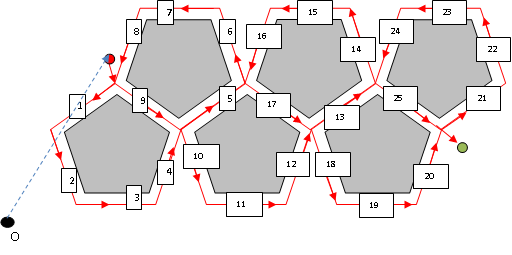
\includegraphics[width=0.8\textwidth]{pentagons.png}
  \caption{Пример составного сегмента резка для шести деталей / контуров}
  \label{fig:6x5}
\end{figure}

Для того,
чтобы можно было описать эти техники резки
в используемой математической модели,
мы вводим новые понятия:

{\it Сегмент резки}
$S = \overrightarrow{M M^*}$
-- это траектория инструмента
от точки врезки
$M$
до соответствующей точки выключения инструмента
$M^*$.

В стандартной технике
сегмент резки содержит ровно один контур детали,
но в общем случае это уже не так.
При мульт-сегментной резки сегмент содержит
только часть контура,
а при мульти-контурной -- несколько контуров
(или их частей).
Рис.~\ref{fig:6x5},
таким образом,
может представлять не только
пример мульти-контурной резки,
но также и один единственный сегмент
в составе некоторой большей задачи резки.

Поскольку сегмент резки по определению содержит
информацию о направлении резки,
нам потребуется ещё одно понятие:

{\it Базовый сегмент}
$B^S$
-- это часть сегмента резки
$S = \overrightarrow{M M^*}$,
без начальной и конечной части
(вспомогательных движений резака,
когда он движется от точки врезки
к собственно контуру и отходит
от вырезанного контура в конце).
Базовый сегмент не содержит информации
о направлении резки
и является чисто геометрическим объектом.

При помощи понятия базового сегмента
оказывается возможным сформулировать
обобщение задачи непрерывной резки:

{\it Сегментная задача непрерывной резки}
(Segment Continuous Cutting Problem, SCCP)
-- это задача резки фиксированного набора
базовых сегментов резки
$SCCP = \left\{B^{S_i}\right\}$.

Описанный в разделе~\ref{sec:ccp-relax}
алгоритм CCP-Relax
естественным образом обобщается
на решение задачи SCCP.

\begin{figure}
  \centering
  \subfloat[Стандартная резка, 45 сегментов]{
    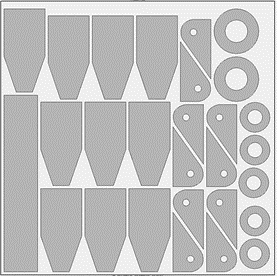
\includegraphics[width=0.45\columnwidth]{nest45.png}
  }
  \subfloat[Мульти-контурная резка, 39 сегментов]{
    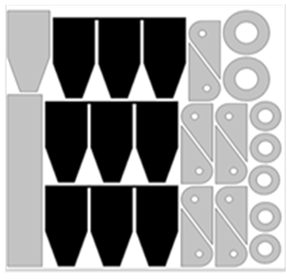
\includegraphics[width=0.47\columnwidth]{nest39.png}
  }
  \caption{{\it Ансамбль} задач сегментной резки}
  \label{fig:gsccp}
\end{figure}

Заметим теперь,
что если задана раскройная карта,
то есть расположение всех деталей и их
граничных контуров,
из неё может быть сгенерирован
целый {\it ансамбль}
наборов базовых сегментов
путём разбиения контуров на сегменты
и объединения нескольких сегментов в один.
См., например,
рис.~\ref{fig:gsccp},
где мульти-контурные сегменты выделены
чёрным цветом.
Это позволяет ещё больше обобщить задачу
и сформулировать новый класс:

{\it Обобщённая задача сегментной резки}
(Generalized Segment Continuous Cutting Problem, GSCCP)
-- {\it ансамбль} нескольких задач сегментной резки
(SCCP)
для одного раскройного плана:
$GSCCP = \left\{ SCCP_i \right\}$.

Введение нового класса задач резки GSCCP
существенно расширяет существующую классификацию
задач маршрутизации инструмента машин термической резки с ЧПУ.
Фактически,
задачи SCCP и GSCCP
являются частными случаями задачи ICP,
содержащими конечное множество базовых
сегментов резки:
$ CCP \subset SCCP \subset GSCCP \subset ICP$.

\subsection*{Общая схема решения задачи GSCCP}

Предполагая ансамбль
$\left\{ SCCP_i \right\}$
наборов базовых сегментов
$SCCP_i = \left\{B^{S_j}\right\}$,
$
i \in \overline{1, T},
j \in \overline{1, K_i}
$
фиксированным,
используем следующую
общую схему решения задачи GSCCP:

\begin{itemize}
  \item
  Каждая из задач $SCCP_i$
  решается независимо
  любым существующим алгоритмом,
  например:
  \begin{enumerate}
    \item
    {\it CCP-Relax},
    описанная в разделе~\ref{sec:ccp-relax} эвристика.
    \item
    {\it DP-GTSP},
    точный алгоритм динамического программирования
    для задач небольшого размера,
    см.~\cite{bi15}.
    \item
    {\it Greedy-GTSP},
    итеративный жадный эвристический алгоритм,
    см.~\cite{bib:greedy}.
  \end{enumerate}
  Для алгоритмов дискретной оптимизации
  контуры деталей предварительно преобразуются
  в конечные множества допустимых точек врезки,
  как показано на рис.~\ref{fig:gtsp425}.

  \item
  Лучшее решение выбирается
  на основе значения целевой функции
  (\ref{air-move-length}).
\end{itemize}

\begin{figure}
  \centering
  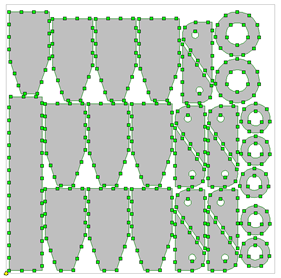
\includegraphics[width=0.5\columnwidth]{gtsp425.png}
  \caption{
    Задача GTSP, полученная по задаче (S)CCP на рис.~\ref{fig:gsccp},\\
    425 точек врезки
  }
  \label{fig:gtsp425}
\end{figure}

Рис.~\ref{fig:gsccp-cut}
показывает решения задач SCCP
с рис.~\ref{fig:gsccp},
полученные при помощи алгоритма
{\it CCP-Relax}.
Легко видеть,
что маршруты действительно различаются.
Более того,
с практической точки зрения,
различие может быть ещё более значительным,
так как маршруты отличаются не только
геометрически,
но и количеством точек врезки,
а эта операция сравнительно дорогая
для современных машин резки с ЧПУ,
как в смысле стоимости,
так и времени работы.

\begin{figure}
  \centering
  \subfloat[Стандартная резка]{
    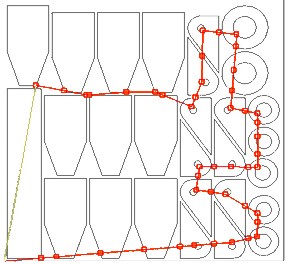
\includegraphics[width=0.45\columnwidth]{cut45.png}
  }
  \subfloat[Мульти-контурная резка]{
    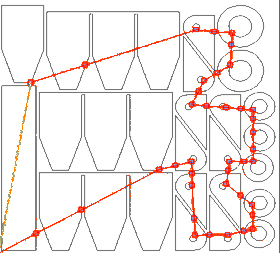
\includegraphics[width=0.47\columnwidth]{cut39.png}
  }
  \caption{Решение задачи GSCCP с рис.~\ref{fig:gsccp}}
  \label{fig:gsccp-cut}
\end{figure}

\section{Численные эксперименты}
\label{sec:calc}

Оценка качества решений,
получаемых алгоритмом CCP-Relax
проводилась на нескольких раскройных планах,
содержащих реальные детали.
В качестве базы сравнения
был взят точный алгоритм
решения задачи GTSP на основе динамического программирования
(см.~\cite{bi15}),
гарантирующий нахождение
наилучшего решения для задач
с небольшим количеством контуров,
а также специализированная версия эвристики
GNLS \cite{GLNS}.

На рис.~\ref{gtsp-path}
представлено точное решение,
при этом видны допустимые точки врезки,
полученные дискретизацией исходных контуров деталей.
На рис.~\ref{ccp-path}
представлено решение задачи CCP,
полученное алгоритмом CCP-Relax.

\begin{figure}
  \begin{center}
    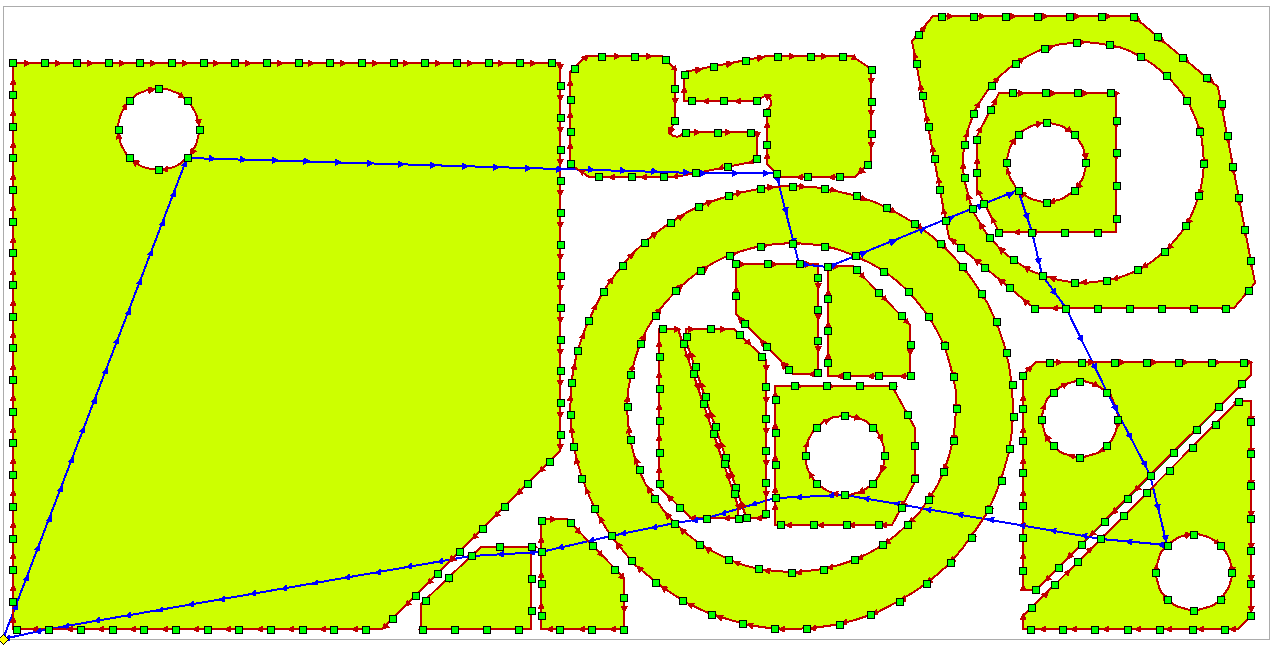
\includegraphics[width=0.95\textwidth]{464-gtsp.png}
  \end{center}
  \caption{Точное решение задачи GTSP, задание №~464}
  \label{gtsp-path}
\end{figure}

\begin{figure}
  \begin{center}
    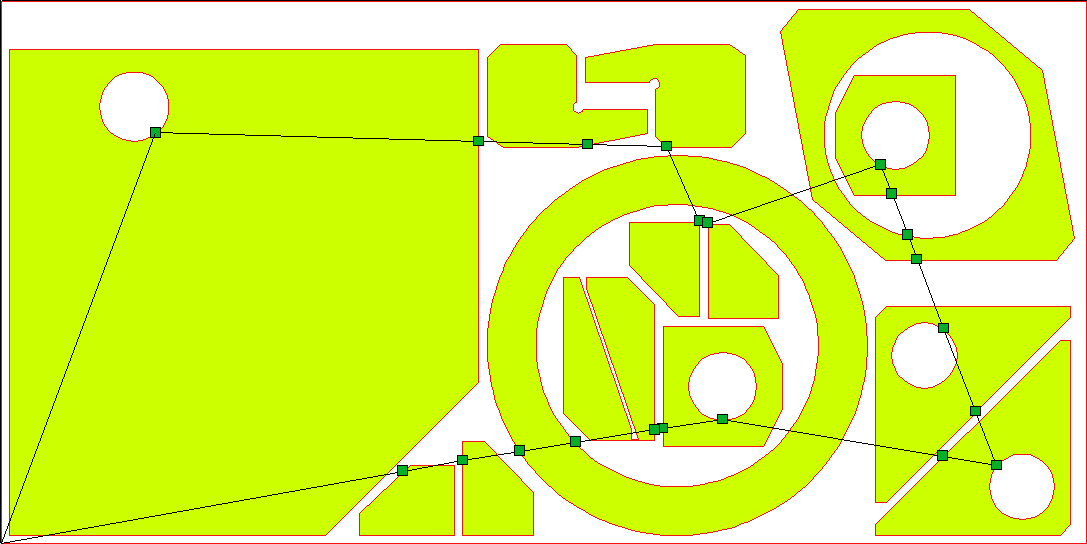
\includegraphics[width=0.95\textwidth]{464-ccp.png}
  \end{center}
  \caption{Решение задачи CCP, задание №~464}
  \label{ccp-path}
\end{figure}

Можно отметить,
что полученные маршруты практически идентичны.
Небольшие отклонения вызваны процессом предварительной дискретизации
(при переводе задачи CCP в GTSP).
Вследствие этого,
алгоритм CCP-Relax формирует прямые сегменты
холостого хода инструмента,
а в случае задачи GTSP
получаются слегка ломаные линии,
что слегка увеличивает результирующую длину маршрута.
Более точно это отражено в табл.~\ref{ccp-vs-gtsp}
для нескольких раскройных планов.

\begin{table}[h]
  \begin{center}
  \begin{tabular}{l*{4}{|r}}
      Задание & № 229 & № 464 & № 3211 & № 20205 \\
      \hline \hline
      Деталей & 11 & 14 & 17 & 115 \\
      \hline
      Контуров & 12 & 21 & 22 & 198 \\
      \hline
      Точек GTSP & 491 & 429 & 493 & 3917 \\
      \hline
      $\mathcal L_{GTSP}$, m & 7.729 & 4.743 & 4.557 & 26.098 \\
      \hline
      $\mathcal L_{CCP}$, m & 7.727 & 4.706 & 4.536 & 25.987 \\
      \hline
  \end{tabular}
  \caption{Сравнение решений задач CCP и GTSP}
  \label{ccp-vs-gtsp}
  \end{center}
\end{table}

На рис.~\ref{large-path}
показано решение задачи CCP
(алгоритмом CCP-Relax)
для раскройного плана на 198 контуров,
когда точное решение не известно.
Вообще,
для задач такого и большего размера
(а именно они представляют практический интерес),
оценка оптимальности решения
представляет собой довольно большие сложности.
Тем не менее,
сравнение с решениями
хорошо исследованной задачи GTSP
вполне применимо для оценки качества решения.
Как известно,
GTSP является NP-сложной
даже на Эвклидовой плоскости
\cite{bib:x103}.

Хотя из общих соображений понятно,
что чем больше ограничений
(имеются в виду ограничения предшествования)
наложено на задачу GTSP,
тем проще её решить,
вопрос влияния уровня вложенности деталей
на границы сложности решений ещё
не достаточно исследовался и заслуживает внимания.
По этому поводу хочется отметить работы
\cite{bib:x104,bib:x105}.
Для двух видов ограничений предшествования
теоретически доказана полиномиальная временная сложность
задачи GTSP.
Один тип описан Е. Баласом в
\cite{bib:x100}
для классической задачи TSP.
Эффективный точный алгоритм для задачи GTSP
с такими ограничениями предшествования
предложен в работах
\cite{bib:x102,ChentsovIII}.
Маршруты,
содержащие ограничения второго вида,
называются квази- и псевдо-пирамидальными.
Эффективные параметрические алгоритмы
решения задачи GTSP
с ограничениями такого вида предложены в
\cite{KhachaiI,KhachayII}.

Ввиду вышеизложенного,
можно заключить,
что алгоритмический анализ
даже задачи GTSP
в приложении к маршрутизации резки
всё ещё является малоисследованной областью.
В частности,
отсутствие эффективных моделей
MILP (Mixed Integer Linear Program)
для задачи GTSP
делает невозможным использование
современных решателей,
таких как Gurobi
\cite{bib:x101}
для построения верхних и нижних границ
и оценки эвристических решений.
Это также представляется перспективным
направлением исследований.


\begin{figure}
  \begin{center}
    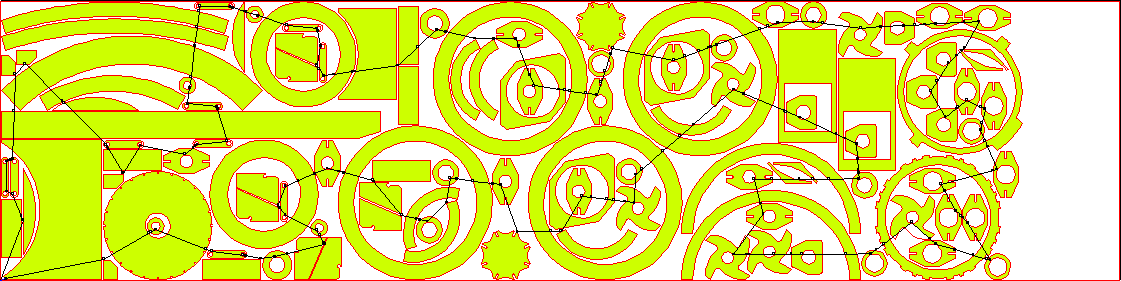
\includegraphics[width=0.9\textwidth]{test5-ccp.png}
  \end{center}
  \caption{Пример решения задачи CCP большого размера, задание № 20205}
  \label{large-path}
\end{figure}

\section{Заключение}
\label{sec:conclude}

\begin{enumerate}
  \item
  Задача минимизации длины холостого хода инструмента
  машин термической резки с ЧПУ
  для задачи непрерывной резки
  сведена к аналогичной задаче,
  не содержащей ограничений предшествования,
  сокращая количество контуров и время работы алгоритма
  \item
  Предложен эвристический алгоритм CCP-Relax
  поиска положений точек врезки в задаче непрерывной резки
  \item
  Доказано, что алгоритм CCP-Relax
  при заданном порядке обхода контуров
  доставляет локальный минимум длины холостого хода
  \item
  Сформулировано несколько легко проверяемых условий,
  при которых решение, полученное алгоритмом CCP-Relax,
  является глобальным минимумом.
  \item
  Алгоритм CCP-Relax
  может применяться также для решения более широкого класса
  задач резки --
  SCCP (Сегментная резка) и
  GSCCP (Обобщённая сегментная резка),
  что в свою очередь является перспективным подходом
  к решению общей задачи
  ICP.
\end{enumerate}

Ближайшим направлением дальнейших исследований
является обобщение алгоритма CCP-Relax
на более практический случай,
когда точки врезки лежат вне контуров деталей
в соответствии с технологическими требованиями
современного оборудования с ЧПУ.

\printbibliography[title=Литература]

\begin{aboutAuthors}

\textbf{Петунин Александр Александрович}~---~д-р техн. наук., доцент;
профессор кафедры информационных технологий и автоматизации проектирования УрФУ.
Число научных публикаций~---~147.
a.a.petunin@urfu.ru,
https://urfu.ru;
Уральский Федеральный университет,
620002, Екатеринбург, Мира, 19.
\smallskip

\textbf{Полищук Ефим Григорьевич}~---~канд. физ-мат. наук, доцент;
старший научный сотрудник
лаборатории оптимального раскроя промышленных материалов и оптимальных маршрутных технологий УрФУ.
Число научных публикаций~---~16.
e.g.polishchuk@urfu.ru,
https://urfu.ru;
Уральский Федеральный университет,
620002, Екатеринбург, Мира, 19.
\smallskip

\textbf{Уколов Станислав Сергеевич}~---~младший научный сотрудник
лаборатории оптимального раскроя промышленных материалов и оптимальных маршрутных технологий УрФУ.
Область научных интересов:
  маршрутизация инструмента машин термической резки с ЧПУ.
Число научных публикаций~---~9.
s.s.ukolov@urfu.ru,
https://urfu.ru;
Уральский Федеральный университет,
620002, Екатеринбург, Мира, 19.
\smallskip

\textbf{Поддержка исследований.}
Работа выполнена при финансовой поддержке Министерства науки и высшего образования РФ,
Государственный контракт № 075-03-2020-582/4.

\end{aboutAuthors}

\end{document}
